\documentclass[12pt,]{article}
\usepackage{lmodern}
\usepackage{amssymb,amsmath}
\usepackage{ifxetex,ifluatex}
\usepackage{fixltx2e} % provides \textsubscript
\ifnum 0\ifxetex 1\fi\ifluatex 1\fi=0 % if pdftex
  \usepackage[T1]{fontenc}
  \usepackage[utf8]{inputenc}
\else % if luatex or xelatex
  \ifxetex
    \usepackage{mathspec}
  \else
    \usepackage{fontspec}
  \fi
  \defaultfontfeatures{Ligatures=TeX,Scale=MatchLowercase}
\fi
% use upquote if available, for straight quotes in verbatim environments
\IfFileExists{upquote.sty}{\usepackage{upquote}}{}
% use microtype if available
\IfFileExists{microtype.sty}{%
\usepackage{microtype}
\UseMicrotypeSet[protrusion]{basicmath} % disable protrusion for tt fonts
}{}
\usepackage[margin=1in]{geometry}
\usepackage{hyperref}
\hypersetup{unicode=true,
            pdftitle={Second BM25 A/B Test Analysis},
            pdfauthor={Chelsy Xie (Analysis \& Report); Erik Bernhardson (Engineering); David Causse (Engineering \& Review); Trey Jones (Engineering \& Review); Mikhail Popov (Review); Deb Tankersley (Product Management)},
            pdfborder={0 0 0},
            breaklinks=true}
\urlstyle{same}  % don't use monospace font for urls
\usepackage{longtable,booktabs}
\usepackage{graphicx,grffile}
\makeatletter
\def\maxwidth{\ifdim\Gin@nat@width>\linewidth\linewidth\else\Gin@nat@width\fi}
\def\maxheight{\ifdim\Gin@nat@height>\textheight\textheight\else\Gin@nat@height\fi}
\makeatother
% Scale images if necessary, so that they will not overflow the page
% margins by default, and it is still possible to overwrite the defaults
% using explicit options in \includegraphics[width, height, ...]{}
\setkeys{Gin}{width=\maxwidth,height=\maxheight,keepaspectratio}
\IfFileExists{parskip.sty}{%
\usepackage{parskip}
}{% else
\setlength{\parindent}{0pt}
\setlength{\parskip}{6pt plus 2pt minus 1pt}
}
\setlength{\emergencystretch}{3em}  % prevent overfull lines
\providecommand{\tightlist}{%
  \setlength{\itemsep}{0pt}\setlength{\parskip}{0pt}}
\setcounter{secnumdepth}{0}
% Redefines (sub)paragraphs to behave more like sections
\ifx\paragraph\undefined\else
\let\oldparagraph\paragraph
\renewcommand{\paragraph}[1]{\oldparagraph{#1}\mbox{}}
\fi
\ifx\subparagraph\undefined\else
\let\oldsubparagraph\subparagraph
\renewcommand{\subparagraph}[1]{\oldsubparagraph{#1}\mbox{}}
\fi

%%% Use protect on footnotes to avoid problems with footnotes in titles
\let\rmarkdownfootnote\footnote%
\def\footnote{\protect\rmarkdownfootnote}

%%% Change title format to be more compact
\usepackage{titling}

% Create subtitle command for use in maketitle
\newcommand{\subtitle}[1]{
  \posttitle{
    \begin{center}\large#1\end{center}
    }
}

\setlength{\droptitle}{-2em}
  \title{Second BM25 A/B Test Analysis}
  \pretitle{\vspace{\droptitle}\centering\huge}
  \posttitle{\par}
  \author{Chelsy Xie (Analysis \& Report) \\ Erik Bernhardson (Engineering) \\ David Causse (Engineering \& Review) \\ Trey Jones (Engineering \& Review) \\ Mikhail Popov (Review) \\ Deb Tankersley (Product Management)}
  \preauthor{\centering\large\emph}
  \postauthor{\par}
  \predate{\centering\large\emph}
  \postdate{\par}
  \date{06 January 2017}

\usepackage[T1]{fontenc}
\usepackage{fontspec}
\setsansfont{Gill Sans}
\DeclareTextCommandDefault{\nobreakspace}{\leavevmode\nobreak\ } 
% ^ http://tex.stackexchange.com/a/66951

\usepackage{pdflscape}
\usepackage{color, colortbl}
\usepackage[dvipsnames]{xcolor}
\definecolor{LightYellow}{rgb}{1.0,1.0,0.702}
\usepackage[font={small,it,sf}]{caption}
\usepackage[font={small,it,sf}]{subcaption}
\usepackage{hyperref}
\usepackage{xeCJK}

\hypersetup{colorlinks=true,linkbordercolor=Blue,linkcolor=Blue,pdfborderstyle={/S/U/W 1}}
\def\UrlFont{\bfseries\color{Blue}}

\begin{document}
\maketitle

\renewcommand{\abstractname}{Executive Summary}

\begin{abstract}
In order to assess the efficacy of BM25 in space-less language, Discovery\textquotesingle s Search team has decided to conduct a second A/B test in Chinese, Japanese and Thai Wikipedias. We observed that the test group that used per-field query builder with incoming links and pageviews as query-independent factors had a much better Zero Result Rate but slightly worse PaulScores, large decrease in clickthrough rate, and fewer users clicked on the first result first, which indicates that we are showing test group users worse results. However, longer dwell-time and fewer query reformulations show that test group users might actually like the results they are getting better than the control group in that respect. We recommend deploying BM25 for all wikis but not reindexing projects in space-less languages for now.
\end{abstract}

\subsection{Background}\label{background}

To improve the relevancy of search results, Discovery's Search team
decided to try a new document-ranking function called
\href{https://en.wikipedia.org/wiki/Okapi_BM25}{Okapi BM25} (BM stands
for Best Matching), and ran an
\href{https://phabricator.wikimedia.org/T143585}{A/B test} from August
30 to September 10 to assess the efficacy of the proposed switch. The
\href{https://wikimedia-research.github.io/Discovery-Search-Test-BM25}{analysis}
showed that BM25 ranking with incoming links and pageviews as
query-independent factors appears to give users results that are more
relevant and that they engage with more.

However, we then
\href{https://phabricator.wikimedia.org/T147008\#2679631}{realized} that
our analysis chain is sub-optimal for space-less language queries, which
will break words on every characters for the plain field. Therefore, we
ran a \href{https://phabricator.wikimedia.org/T147495}{second A/B test}
for Chinese, Japanese and Thai Wikipedias to test whether the new
per-field BM25 builder is sufficiently worse with those languages. We
are primarily interested in:

\begin{itemize}
\tightlist
\item
  \textbf{Zero results rate}, the proportion of searches that yielded
  zero results (smaller is usually better)
\item
  \textbf{Users' engagement} with the search results, measured as the
  clickthrough rate (bigger is better)
\item
  \textbf{PaulScore}, a metric of search results' relevancy that relies
  on the position of the clicked result{[}s{]} (bigger is better); see
  \href{https://wikimedia-research.github.io/Discovery-Search-Test-BM25/\#paulscore_definition}{PaulScore
  Definition} for more details
\item
  \textbf{Query reformulation} -- one way to think about the strength of
  our search engine is how many times the user reformulates their query;
  if a user in the test group has to reformulate their query many more
  times to get the results they are interested in, then maybe the change
  is for the worse
\item
  \textbf{Dwell Time}, the time (seconds) that users stayed on the pages
  they visited by clicking on the search results (bigger is better)
\item
  \textbf{Scroll} -- if users scroll on the visited page, they are more
  likely to engage with the contents
\end{itemize}

\subsection{Data}\label{data}

For Chinese Wikipedia (zhwiki) and Japanese Wikipedia (jawiki), users
had a 1 in 16 chance of being selected for anonymous tracking according
to our
\href{https://meta.wikimedia.org/w/index.php?title=Schema:TestSearchSatisfaction2\&id=15922352}{TestSearchSatisfaction2
\#15922352} event logging schema. Those users who were randomly selected
to have their sessions anonymously tracked then had a 12 in 13 chance of
being selected for the BM25 test. For Thai Wikipedia (thwiki), users had
a 1 in 5 chance of being selected for search satisfaction tracking and
then had a 38 in 39 chance of being selected for the BM25 test due to
fewer visitors to that particular project. The sampled sessions were
evenly put into a control group (tf-idf) and a test group (using
per-field query builder with incoming links and pageviews as QIFs); see
the
\href{https://wikimedia-research.github.io/Discovery-Search-Test-BM25/\#data}{first
BM25 test report} for more details. The test was deployed on October
27th and ran for a week for zhwiki and jawiki, but until November 15th
for thwiki specifically.

The full-text (as opposed to auto-complete) searching event logging data
was extracted from the database using this
\href{https://github.com/wikimedia-research/Discovery-Search-2ndTest-BM25_jazhth/blob/master/data.R}{script}.
We collected a total of 230.2K events from 36.1K unique sessions. See
Table 1 for counts broken down by wiki and test group.

\begin{longtable}[]{@{}llrr@{}}
\toprule
\begin{minipage}[b]{0.08\columnwidth}\raggedright\strut
wiki\strut
\end{minipage} & \begin{minipage}[b]{0.55\columnwidth}\raggedright\strut
Test group\strut
\end{minipage} & \begin{minipage}[b]{0.13\columnwidth}\raggedleft\strut
Search sessions\strut
\end{minipage} & \begin{minipage}[b]{0.13\columnwidth}\raggedleft\strut
Events recorded\strut
\end{minipage}\tabularnewline
\midrule
\endhead
\begin{minipage}[t]{0.08\columnwidth}\raggedright\strut
jawiki\strut
\end{minipage} & \begin{minipage}[t]{0.55\columnwidth}\raggedright\strut
Control Group (tf--idf)\strut
\end{minipage} & \begin{minipage}[t]{0.13\columnwidth}\raggedleft\strut
7,579\strut
\end{minipage} & \begin{minipage}[t]{0.13\columnwidth}\raggedleft\strut
54,261\strut
\end{minipage}\tabularnewline
\begin{minipage}[t]{0.08\columnwidth}\raggedright\strut
jawiki\strut
\end{minipage} & \begin{minipage}[t]{0.55\columnwidth}\raggedright\strut
Using per-field query builder with incoming links and pageviews as
QIFs\strut
\end{minipage} & \begin{minipage}[t]{0.13\columnwidth}\raggedleft\strut
7,610\strut
\end{minipage} & \begin{minipage}[t]{0.13\columnwidth}\raggedleft\strut
59,808\strut
\end{minipage}\tabularnewline
\begin{minipage}[t]{0.08\columnwidth}\raggedright\strut
thwiki\strut
\end{minipage} & \begin{minipage}[t]{0.55\columnwidth}\raggedright\strut
Control Group (tf--idf)\strut
\end{minipage} & \begin{minipage}[t]{0.13\columnwidth}\raggedleft\strut
3,889\strut
\end{minipage} & \begin{minipage}[t]{0.13\columnwidth}\raggedleft\strut
18,954\strut
\end{minipage}\tabularnewline
\begin{minipage}[t]{0.08\columnwidth}\raggedright\strut
thwiki\strut
\end{minipage} & \begin{minipage}[t]{0.55\columnwidth}\raggedright\strut
Using per-field query builder with incoming links and pageviews as
QIFs\strut
\end{minipage} & \begin{minipage}[t]{0.13\columnwidth}\raggedleft\strut
4,055\strut
\end{minipage} & \begin{minipage}[t]{0.13\columnwidth}\raggedleft\strut
21,217\strut
\end{minipage}\tabularnewline
\begin{minipage}[t]{0.08\columnwidth}\raggedright\strut
zhwiki\strut
\end{minipage} & \begin{minipage}[t]{0.55\columnwidth}\raggedright\strut
Control Group (tf--idf)\strut
\end{minipage} & \begin{minipage}[t]{0.13\columnwidth}\raggedleft\strut
6,510\strut
\end{minipage} & \begin{minipage}[t]{0.13\columnwidth}\raggedleft\strut
37,561\strut
\end{minipage}\tabularnewline
\begin{minipage}[t]{0.08\columnwidth}\raggedright\strut
zhwiki\strut
\end{minipage} & \begin{minipage}[t]{0.55\columnwidth}\raggedright\strut
Using per-field query builder with incoming links and pageviews as
QIFs\strut
\end{minipage} & \begin{minipage}[t]{0.13\columnwidth}\raggedleft\strut
6,478\strut
\end{minipage} & \begin{minipage}[t]{0.13\columnwidth}\raggedleft\strut
38,382\strut
\end{minipage}\tabularnewline
\begin{minipage}[t]{0.08\columnwidth}\raggedright\strut
All Wikis\strut
\end{minipage} & \begin{minipage}[t]{0.55\columnwidth}\raggedright\strut
Total\strut
\end{minipage} & \begin{minipage}[t]{0.13\columnwidth}\raggedleft\strut
36,121\strut
\end{minipage} & \begin{minipage}[t]{0.13\columnwidth}\raggedleft\strut
230,183\strut
\end{minipage}\tabularnewline
\bottomrule
\end{longtable}

\textbf{Table 1}: Counts of sessions anonymously tracked and events
collected during the second A/B test (Oct 27 - Nov 15).

An issue we noticed with the event logging is that when the user goes to
the next page of search results or clicks the Back button after visiting
a search result, a new page ID is generated for the search results page.
The page ID is how we connect click events to search result page events.
There is currently a Phabricator ticket
(\href{https://phabricator.wikimedia.org/T146337}{T146337}) for
addressing these issues. For this analysis, we de-duplicated by
connecting search engine results page (searchResultPage) events that
have the exact same search query, and then connected click events
together based on the searchResultPage connectivity.

After de-duplicating, we collapsed 213.4K (searchResultPage and click)
events into 64.5K searches. See Table 2 for counts broken down by wiki
and test group.

\begin{longtable}[]{@{}llrrr@{}}
\toprule
\begin{minipage}[b]{0.07\columnwidth}\raggedright\strut
wiki\strut
\end{minipage} & \begin{minipage}[b]{0.46\columnwidth}\raggedright\strut
Test group\strut
\end{minipage} & \begin{minipage}[b]{0.11\columnwidth}\raggedleft\strut
Search sessions\strut
\end{minipage} & \begin{minipage}[b]{0.12\columnwidth}\raggedleft\strut
Searches recorded\strut
\end{minipage} & \begin{minipage}[b]{0.11\columnwidth}\raggedleft\strut
Events recorded\strut
\end{minipage}\tabularnewline
\midrule
\endhead
\begin{minipage}[t]{0.07\columnwidth}\raggedright\strut
jawiki\strut
\end{minipage} & \begin{minipage}[t]{0.46\columnwidth}\raggedright\strut
Control Group (tf--idf)\strut
\end{minipage} & \begin{minipage}[t]{0.11\columnwidth}\raggedleft\strut
7,579\strut
\end{minipage} & \begin{minipage}[t]{0.12\columnwidth}\raggedleft\strut
13,839\strut
\end{minipage} & \begin{minipage}[t]{0.11\columnwidth}\raggedleft\strut
50,845\strut
\end{minipage}\tabularnewline
\begin{minipage}[t]{0.07\columnwidth}\raggedright\strut
jawiki\strut
\end{minipage} & \begin{minipage}[t]{0.46\columnwidth}\raggedright\strut
Using per-field query builder with incoming links and pageviews as
QIFs\strut
\end{minipage} & \begin{minipage}[t]{0.11\columnwidth}\raggedleft\strut
7,610\strut
\end{minipage} & \begin{minipage}[t]{0.12\columnwidth}\raggedleft\strut
13,982\strut
\end{minipage} & \begin{minipage}[t]{0.11\columnwidth}\raggedleft\strut
56,097\strut
\end{minipage}\tabularnewline
\begin{minipage}[t]{0.07\columnwidth}\raggedright\strut
thwiki\strut
\end{minipage} & \begin{minipage}[t]{0.46\columnwidth}\raggedright\strut
Control Group (tf--idf)\strut
\end{minipage} & \begin{minipage}[t]{0.11\columnwidth}\raggedleft\strut
3,889\strut
\end{minipage} & \begin{minipage}[t]{0.12\columnwidth}\raggedleft\strut
7,005\strut
\end{minipage} & \begin{minipage}[t]{0.11\columnwidth}\raggedleft\strut
16,379\strut
\end{minipage}\tabularnewline
\begin{minipage}[t]{0.07\columnwidth}\raggedright\strut
thwiki\strut
\end{minipage} & \begin{minipage}[t]{0.46\columnwidth}\raggedright\strut
Using per-field query builder with incoming links and pageviews as
QIFs\strut
\end{minipage} & \begin{minipage}[t]{0.11\columnwidth}\raggedleft\strut
4,055\strut
\end{minipage} & \begin{minipage}[t]{0.12\columnwidth}\raggedleft\strut
7,086\strut
\end{minipage} & \begin{minipage}[t]{0.11\columnwidth}\raggedleft\strut
18,481\strut
\end{minipage}\tabularnewline
\begin{minipage}[t]{0.07\columnwidth}\raggedright\strut
zhwiki\strut
\end{minipage} & \begin{minipage}[t]{0.46\columnwidth}\raggedright\strut
Control Group (tf--idf)\strut
\end{minipage} & \begin{minipage}[t]{0.11\columnwidth}\raggedleft\strut
6,510\strut
\end{minipage} & \begin{minipage}[t]{0.12\columnwidth}\raggedleft\strut
11,450\strut
\end{minipage} & \begin{minipage}[t]{0.11\columnwidth}\raggedleft\strut
35,262\strut
\end{minipage}\tabularnewline
\begin{minipage}[t]{0.07\columnwidth}\raggedright\strut
zhwiki\strut
\end{minipage} & \begin{minipage}[t]{0.46\columnwidth}\raggedright\strut
Using per-field query builder with incoming links and pageviews as
QIFs\strut
\end{minipage} & \begin{minipage}[t]{0.11\columnwidth}\raggedleft\strut
6,478\strut
\end{minipage} & \begin{minipage}[t]{0.12\columnwidth}\raggedleft\strut
11,173\strut
\end{minipage} & \begin{minipage}[t]{0.11\columnwidth}\raggedleft\strut
36,373\strut
\end{minipage}\tabularnewline
\begin{minipage}[t]{0.07\columnwidth}\raggedright\strut
All Wikis\strut
\end{minipage} & \begin{minipage}[t]{0.46\columnwidth}\raggedright\strut
Total\strut
\end{minipage} & \begin{minipage}[t]{0.11\columnwidth}\raggedleft\strut
36,121\strut
\end{minipage} & \begin{minipage}[t]{0.12\columnwidth}\raggedleft\strut
64,535\strut
\end{minipage} & \begin{minipage}[t]{0.11\columnwidth}\raggedleft\strut
213,437\strut
\end{minipage}\tabularnewline
\bottomrule
\end{longtable}

\textbf{Table 2}: After searchResultPage De-duplication, Counts of
sessions anonymously tracked and events collected during the second A/B
test (Oct 27 - Nov 15).

There are 22.1K visitPage events (When the user clicks a link in the
results a visitPage event is created). See Table 3 for counts broken
down by wiki and test group.

\begin{longtable}[]{@{}llr@{}}
\toprule
\begin{minipage}[b]{0.10\columnwidth}\raggedright\strut
wiki\strut
\end{minipage} & \begin{minipage}[b]{0.67\columnwidth}\raggedright\strut
Test group\strut
\end{minipage} & \begin{minipage}[b]{0.14\columnwidth}\raggedleft\strut
Visited pages\strut
\end{minipage}\tabularnewline
\midrule
\endhead
\begin{minipage}[t]{0.10\columnwidth}\raggedright\strut
jawiki\strut
\end{minipage} & \begin{minipage}[t]{0.67\columnwidth}\raggedright\strut
Control Group (tf--idf)\strut
\end{minipage} & \begin{minipage}[t]{0.14\columnwidth}\raggedleft\strut
5,431\strut
\end{minipage}\tabularnewline
\begin{minipage}[t]{0.10\columnwidth}\raggedright\strut
jawiki\strut
\end{minipage} & \begin{minipage}[t]{0.67\columnwidth}\raggedright\strut
Using per-field query builder with incoming links and pageviews as
QIFs\strut
\end{minipage} & \begin{minipage}[t]{0.14\columnwidth}\raggedleft\strut
5,954\strut
\end{minipage}\tabularnewline
\begin{minipage}[t]{0.10\columnwidth}\raggedright\strut
thwiki\strut
\end{minipage} & \begin{minipage}[t]{0.67\columnwidth}\raggedright\strut
Control Group (tf--idf)\strut
\end{minipage} & \begin{minipage}[t]{0.14\columnwidth}\raggedleft\strut
1,554\strut
\end{minipage}\tabularnewline
\begin{minipage}[t]{0.10\columnwidth}\raggedright\strut
thwiki\strut
\end{minipage} & \begin{minipage}[t]{0.67\columnwidth}\raggedright\strut
Using per-field query builder with incoming links and pageviews as
QIFs\strut
\end{minipage} & \begin{minipage}[t]{0.14\columnwidth}\raggedleft\strut
1,776\strut
\end{minipage}\tabularnewline
\begin{minipage}[t]{0.10\columnwidth}\raggedright\strut
zhwiki\strut
\end{minipage} & \begin{minipage}[t]{0.67\columnwidth}\raggedright\strut
Control Group (tf--idf)\strut
\end{minipage} & \begin{minipage}[t]{0.14\columnwidth}\raggedleft\strut
3,591\strut
\end{minipage}\tabularnewline
\begin{minipage}[t]{0.10\columnwidth}\raggedright\strut
zhwiki\strut
\end{minipage} & \begin{minipage}[t]{0.67\columnwidth}\raggedright\strut
Using per-field query builder with incoming links and pageviews as
QIFs\strut
\end{minipage} & \begin{minipage}[t]{0.14\columnwidth}\raggedleft\strut
3,807\strut
\end{minipage}\tabularnewline
\begin{minipage}[t]{0.10\columnwidth}\raggedright\strut
All Wikis\strut
\end{minipage} & \begin{minipage}[t]{0.67\columnwidth}\raggedright\strut
Total\strut
\end{minipage} & \begin{minipage}[t]{0.14\columnwidth}\raggedleft\strut
22,113\strut
\end{minipage}\tabularnewline
\bottomrule
\end{longtable}

\textbf{Table 3}: Counts of visited pages from search sessions
anonymously tracked during the second A/B test (Oct 27 - Nov 15).

\subsection{Results}\label{results}

\subsubsection{Zero Results Rate}\label{zero-results-rate}

In Figure 1, we see that the test group that used BM25 with incoming
links and pageviews as query-independent factors had a significantly
lower zero results rate (ZRR). Smaller ZRR is usually better, but
looking at the \protect\hyperlink{paulscore}{PaulScore},
\protect\hyperlink{engagement}{engagement} and
\protect\hyperlink{first_clicked_resultux2019s_position}{First Clicked
Result's Position}, we doubt that it came at the cost of relevance and
engagement with the results. Figure 2 shows that zhwiki had the largest
ZRR difference between control and test group.

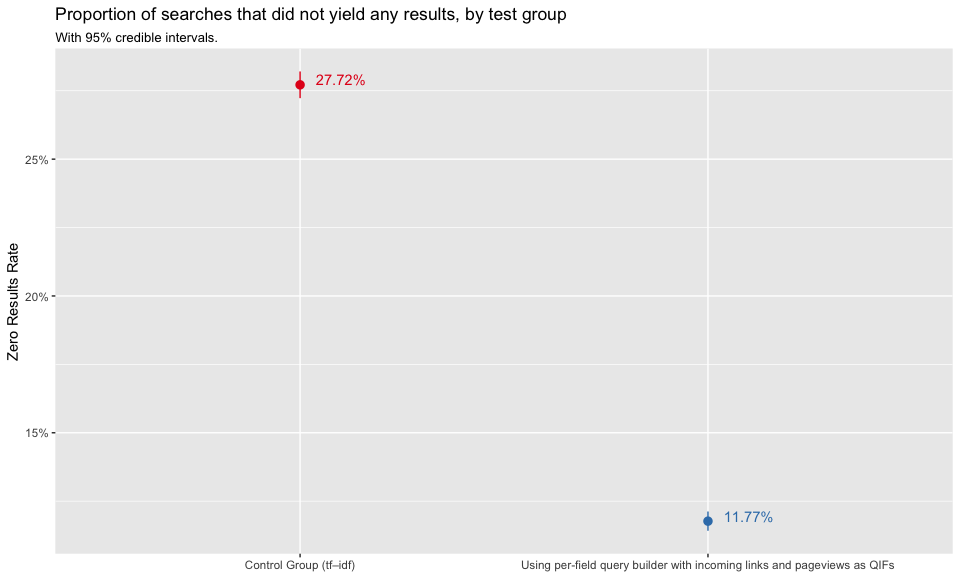
\includegraphics{report_files/figure-latex/zrr_eda-1.pdf}

\textbf{Figure 1}: Zero results rate is the proportion of searches in
which the user received zero results. Broken down by test group.

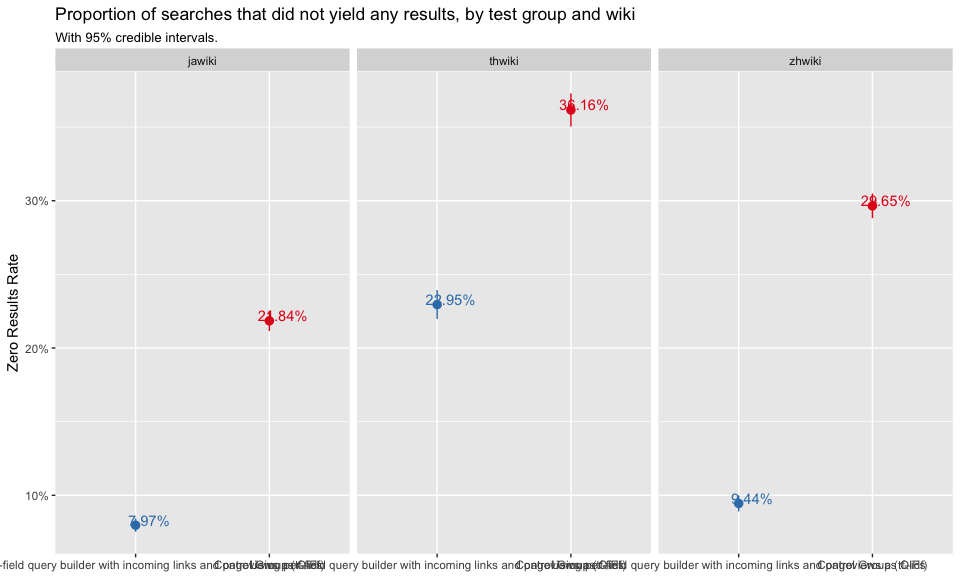
\includegraphics{report_files/figure-latex/zrr_eda2-1.pdf}

\textbf{Figure 2}: Zero results rate is the proportion of searches in
which the user received zero results. Broken down by test group and
wiki.

\hypertarget{paulscore}{\subsubsection{PaulScore}\label{paulscore}}

In Figure 3, we see that the test group had slightly lower PaulScores,
which indicates that the results were less relevant. The difference is
not significant when F = 0.9. This make sense because the smaller the
value of scoring factor, the more weight put on the first few results,
with lower ranking results counting for almost nothing. F=0.9 takes into
account the broadest range of result rankings, and thus is less likely
to change as dramatically. Figure 4 shows that zhwiki had the largest
PaulScore differences between control and test group.

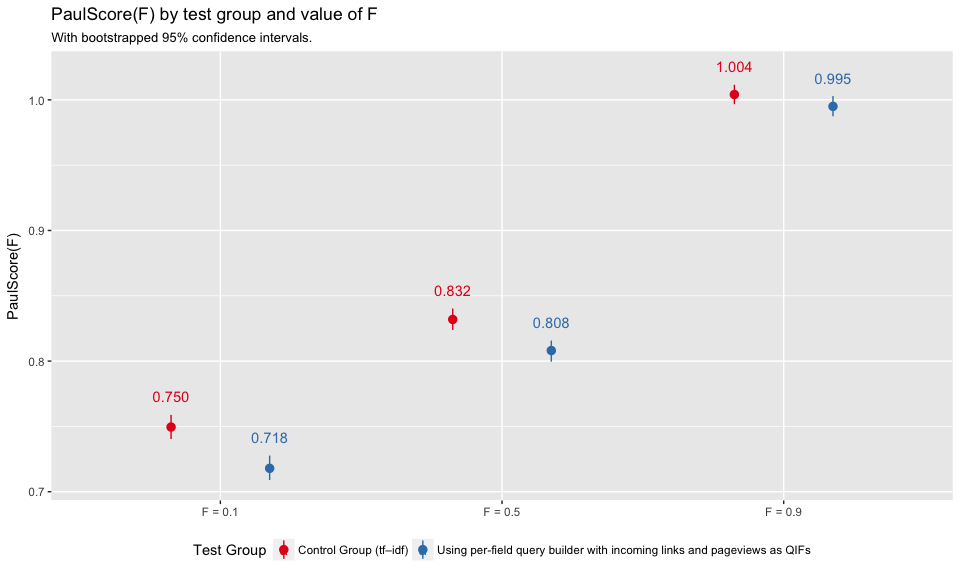
\includegraphics{report_files/figure-latex/paulscores_eda-1.pdf}

\textbf{Figure 3}: Average per-group PaulScore for various values of F
(0.1, 0.5, and 0.9) with bootstrapped confidence intervals.

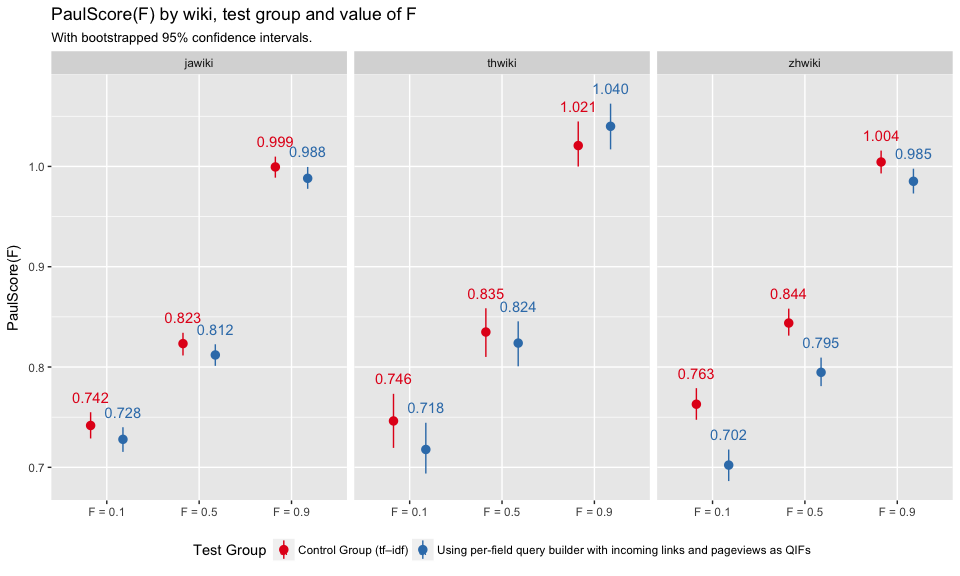
\includegraphics{report_files/figure-latex/paulscores_eda2-1.pdf}

\textbf{Figure 4}: Average per-group PaulScore for various values of F
(0.1, 0.5, and 0.9) with bootstrapped confidence intervals. Broken down
by test group and wiki.

\hypertarget{engagement}{\subsubsection{Engagement}\label{engagement}}

In Figure 5, we see that the test group had a significantly lower
clickthrough rate, which means users are less engaged with their search
results. Again, zhwiki shows the largest discrepancy between control and
test group in Figure 6.

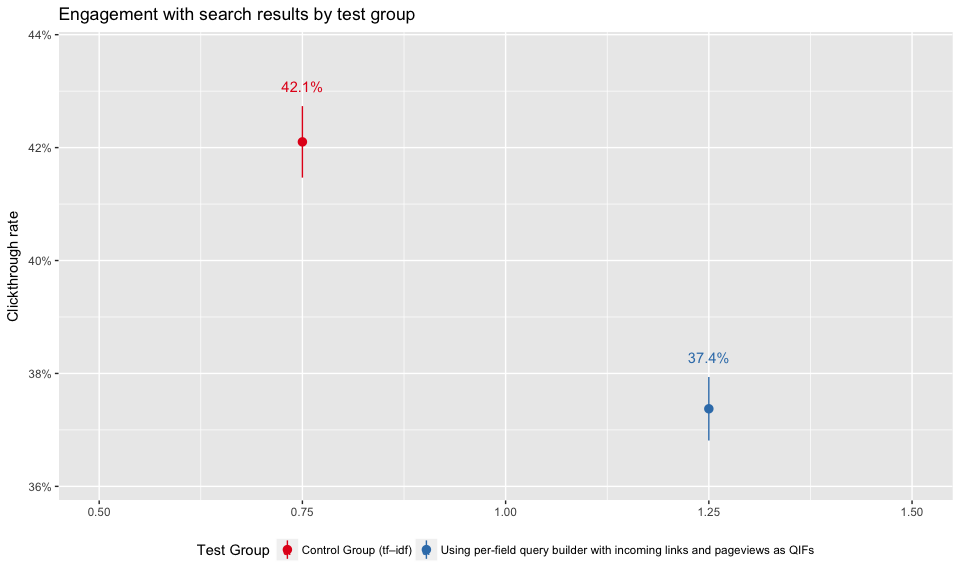
\includegraphics{report_files/figure-latex/engagement_overall_eda-1.pdf}

\textbf{Figure 5}: Clickthrough rates of test groups.

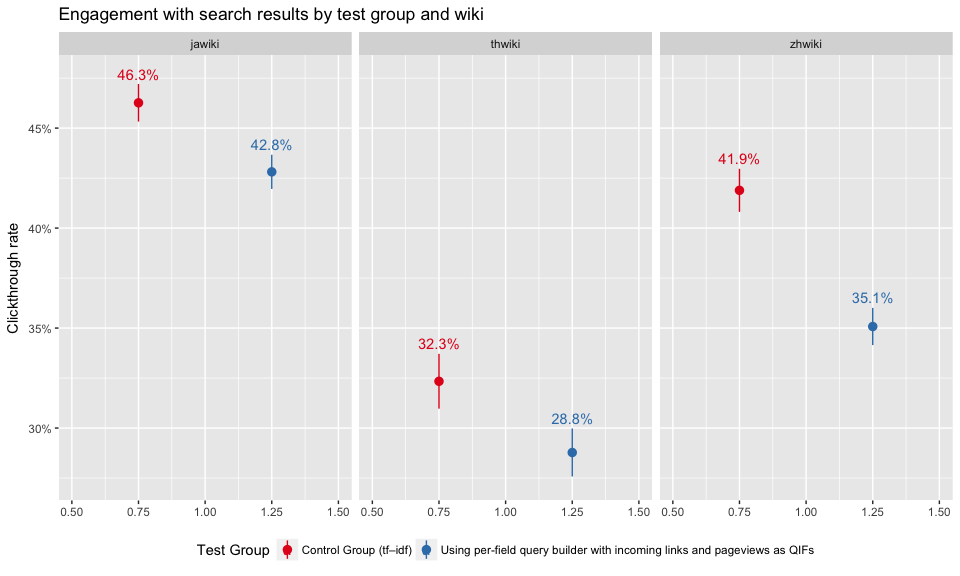
\includegraphics{report_files/figure-latex/engagement_overall_eda2-1.pdf}

\textbf{Figure 6}: Clickthrough rates broken down by test group and
wiki.

\subsubsection{First Clicked Result's
Position}\label{first-clicked-results-position}

In Figure 7, we see that test group users were less likely to click on
the first search result first than the control group. Figure 8 shows
that only zhwiki users first clicked on the first result at a
significantly lower rate, which indicates that the results were less
relevant.

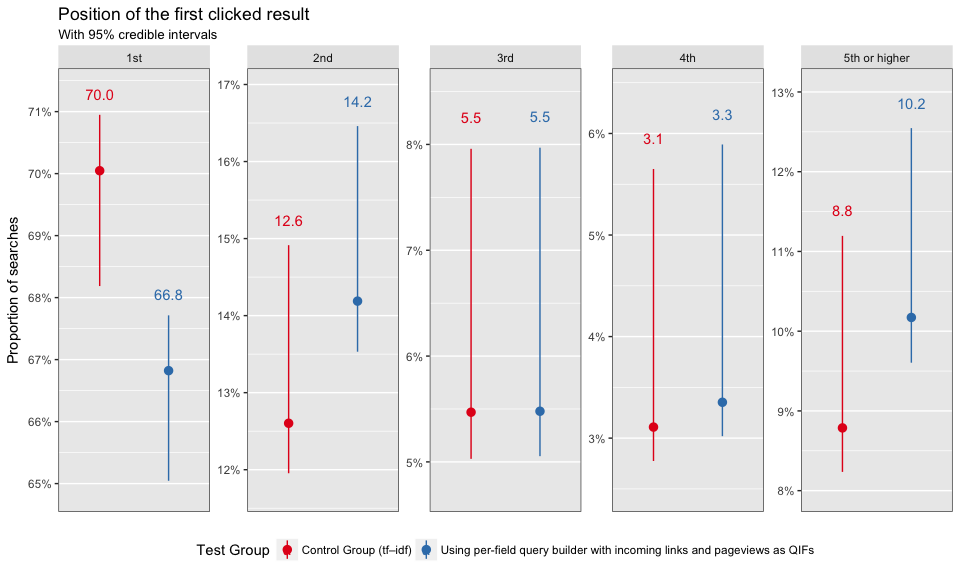
\includegraphics{report_files/figure-latex/first_clicked_position_eda-1.pdf}

\textbf{Figure 7}: First clicked result's position by test group.

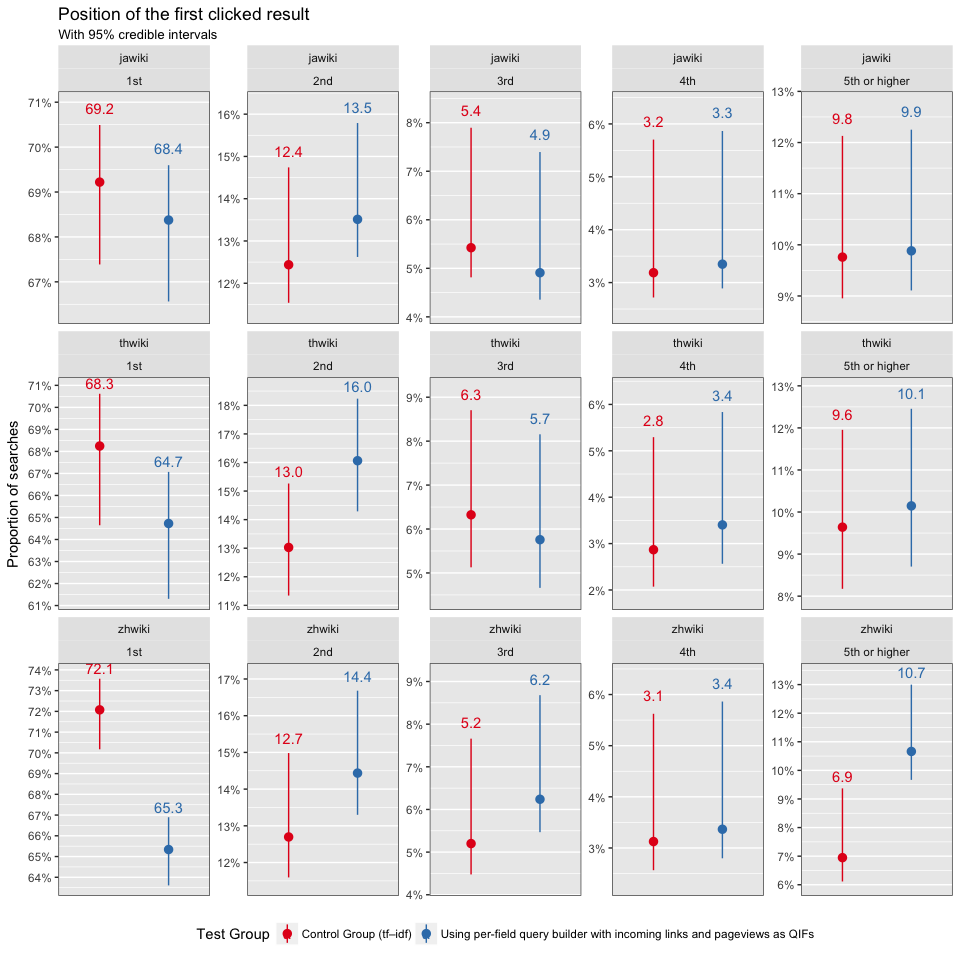
\includegraphics{report_files/figure-latex/first_clicked_position_eda2-1.pdf}

\textbf{Figure 8}: First clicked result's position by test group and
wiki.

\subsubsection{Dwell Time per Visited
Page}\label{dwell-time-per-visited-page}

Figures 9 and 10 show the survival curve for each test group and wiki.
Except zhwiki, users are more likely to stay longer on visited pages,
which implies the results in test group are more relevant for jawiki and
thwiki.

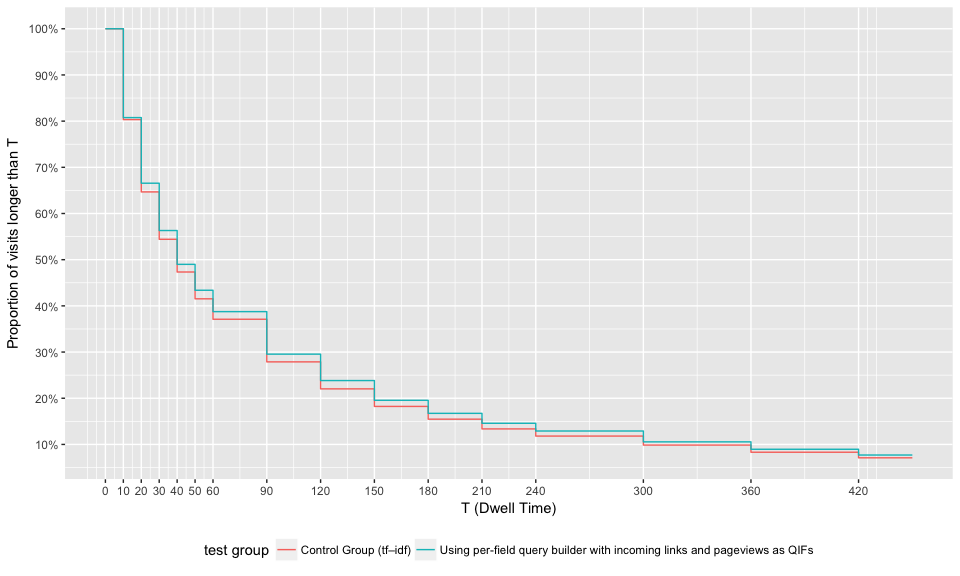
\includegraphics{report_files/figure-latex/dwell_time_eda-1.pdf}

\textbf{Figure 9}: At time T, at most P\% of users still stay on their
visited pages. Broken down by test group.

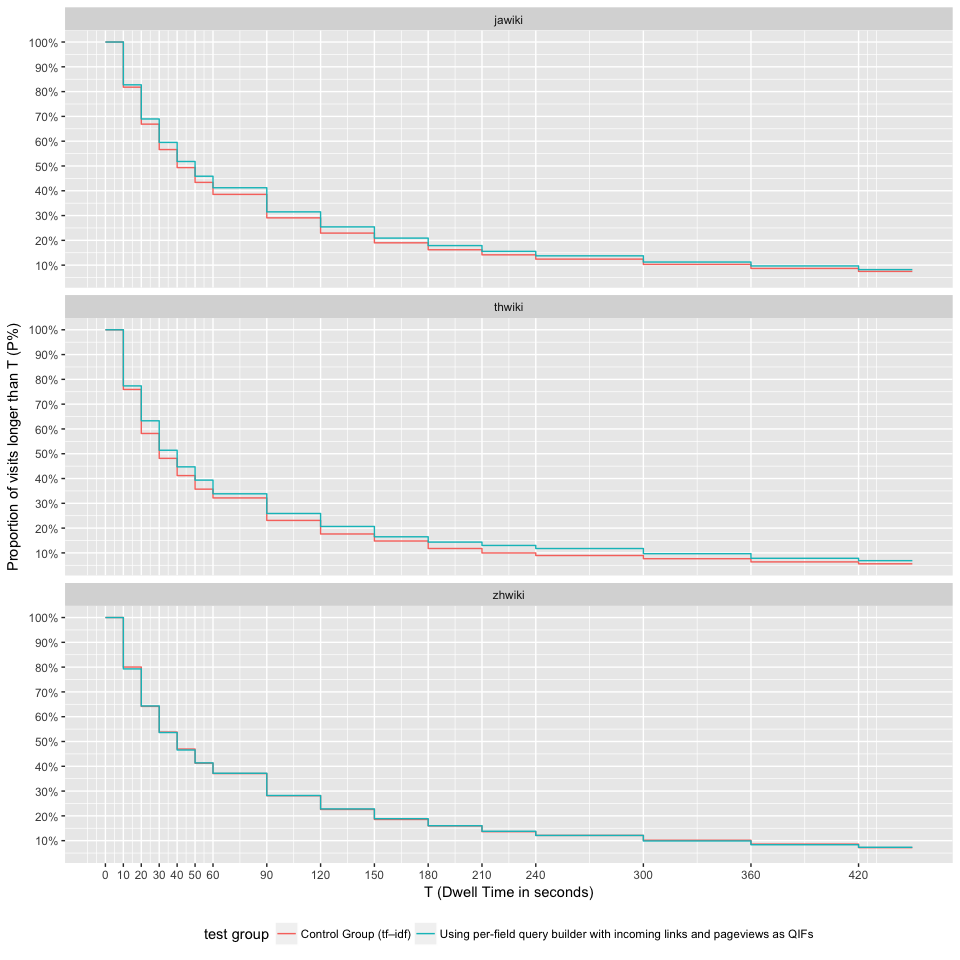
\includegraphics{report_files/figure-latex/dwell_time_eda_wiki-1.pdf}

\textbf{Figure 10}: At time T, at most P\% of users still stay on their
visited pages. Broken down by test group and wiki.

\subsubsection{Scroll}\label{scroll}

In Figures 11 and 12, we can see that users in the test group are more
likely to scroll on the visited pages, but the differences are not
statistically significant.

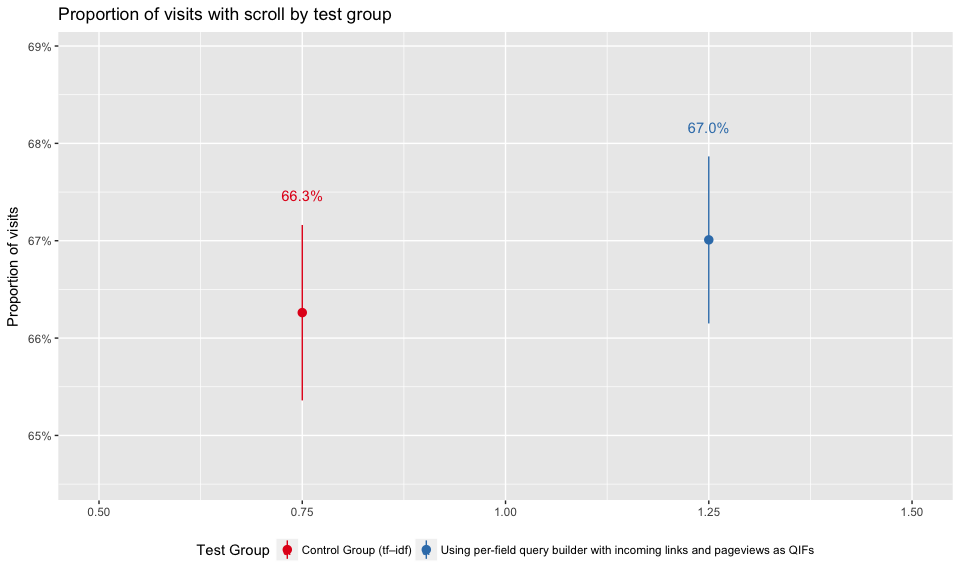
\includegraphics{report_files/figure-latex/scroll_eda-1.pdf}

\textbf{Figure 11}: Proportion of visited pages with scroll by test
group.

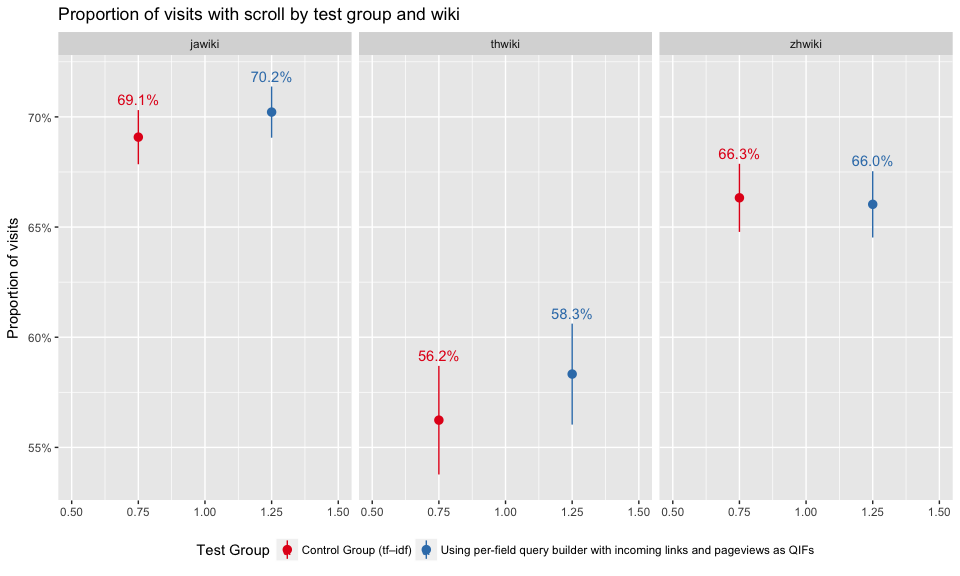
\includegraphics{report_files/figure-latex/scroll_eda_wiki-1.pdf}

\textbf{Figure 12}: Proportion of visited pages with scroll by test
group and wiki.

\subsubsection{Query Reformulation}\label{query-reformulation}

First, we tokenized queries from zhwiki, jawiki and thwiki with
\href{https://github.com/fxsjy/jieba}{jieba},
\href{https://pypi.python.org/pypi/tinysegmenter}{tinysegmenter} and
\href{https://www.elastic.co/guide/en/elasticsearch/reference/current/docs-termvectors.html}{elasticsearch
termvectors api} separately. Then we filter out
\href{https://github.com/6/stopwords-json}{stop words}.

We consider two queries as a reformulation if 1) they are from the same
search session and share at least one result, or 2) they are from the
same search session and share at least one word.

We grouped connected searches together using the rules above, then we
have 51354 total search groups.

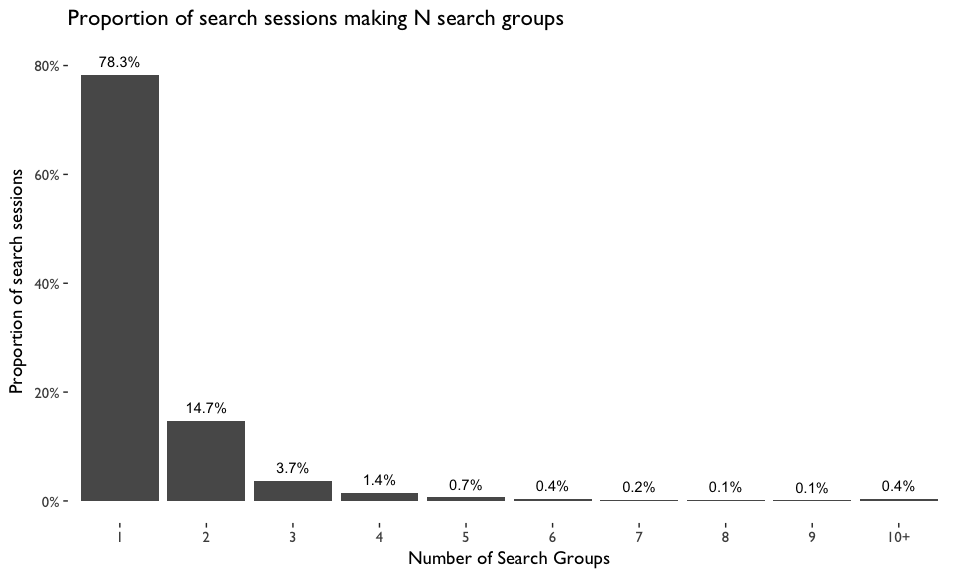
\includegraphics{report_files/figure-latex/reform_n_search_group-1.pdf}

\textbf{Figure 13}: Proportion of search sessions making N search
groups. A search group is a group of searches from the same search
session, in which one search is connected with at least another one if
they share at least one common word or at least one common result.

In Figure 14 and Figure 16, we can see that test group users are less
likely to reformulate their queries. Figure 15 and Figure 17 show that
zhwiki had the largest discrepancy between control and test group.

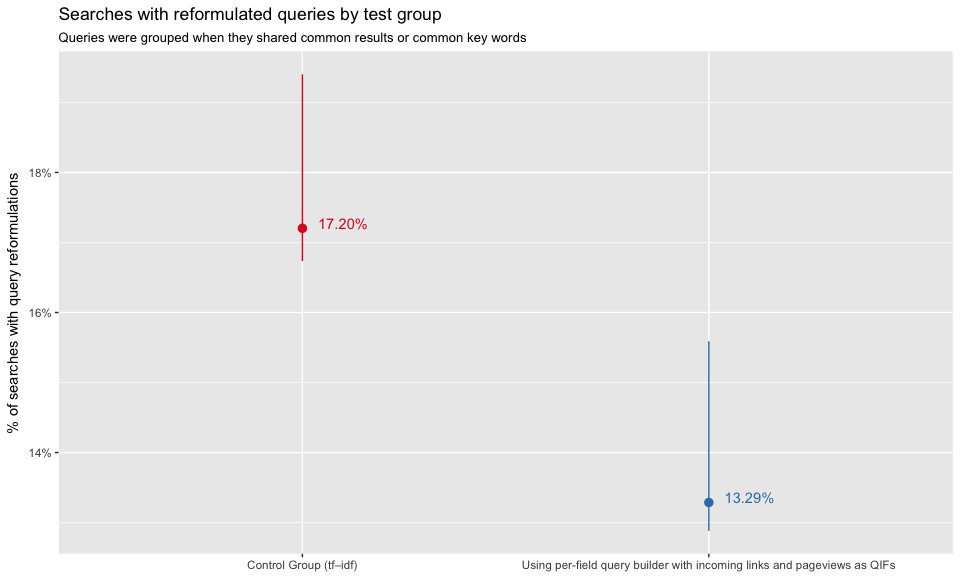
\includegraphics{report_files/figure-latex/reform_eda1-1.pdf}

\textbf{Figure 14}: Proportions of searches where user reformulated
their query.

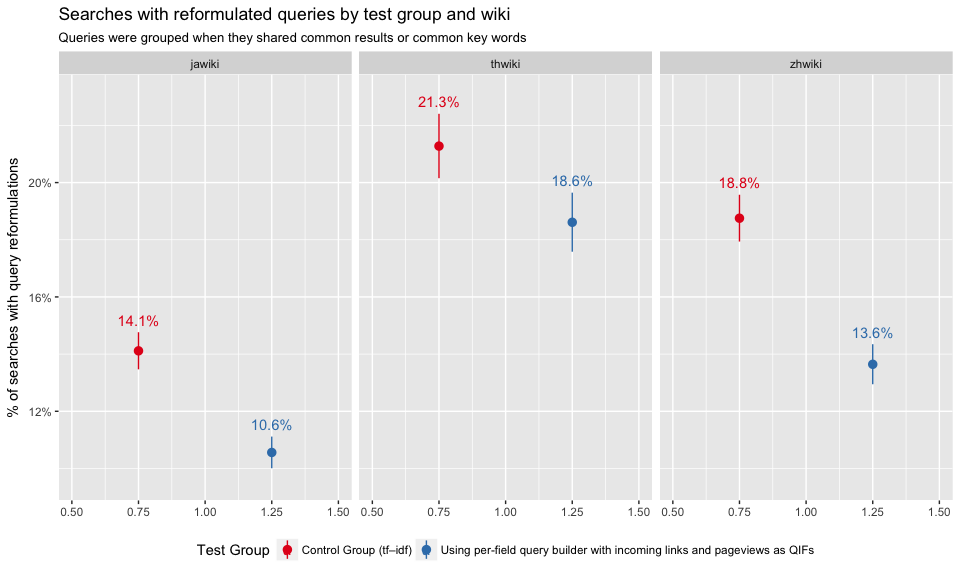
\includegraphics{report_files/figure-latex/reform_eda1_wiki-1.pdf}

\textbf{Figure 15}: Proportions of searches where user reformulated
their query. Broken down by wiki.

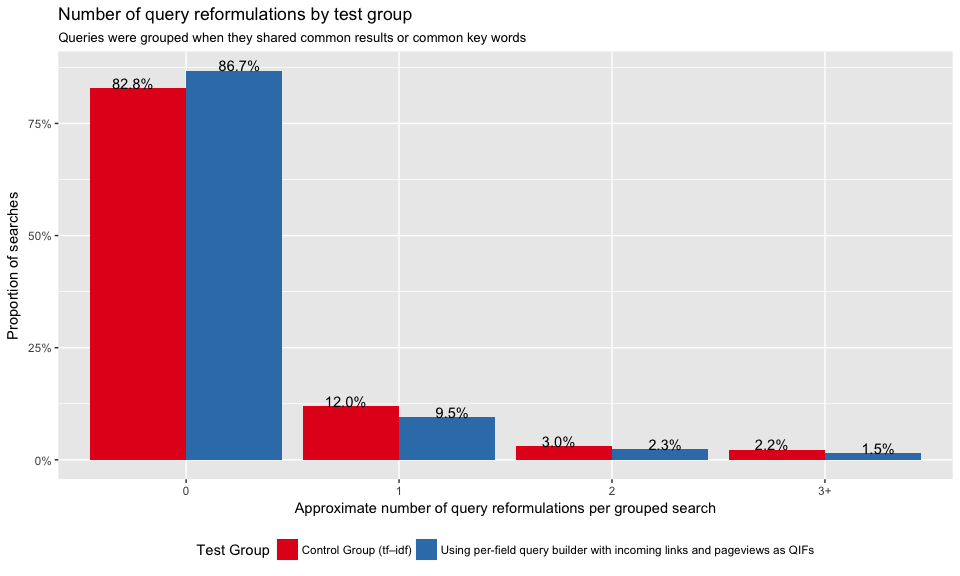
\includegraphics{report_files/figure-latex/reform_eda2-1.pdf}

\textbf{Figure 16}: Proportions of searches with 0, 1, 2, and 3+ query
reformulations.

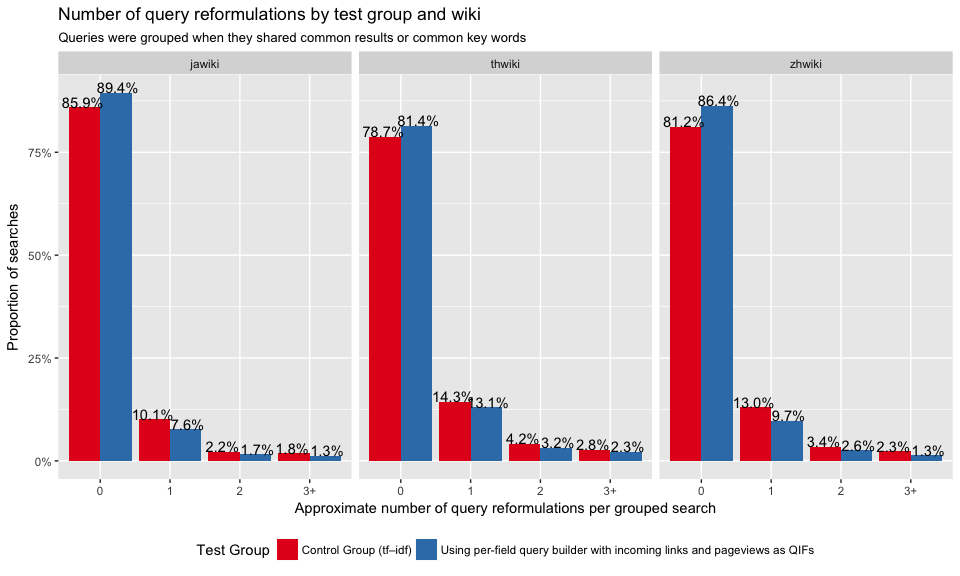
\includegraphics{report_files/figure-latex/reform_eda2_wiki-1.pdf}

\textbf{Figure 17}: Proportions of searches with 0, 1, 2, and 3+ query
reformulations. Broken down by wiki.

\subsection{Conclusion and Discussion}\label{conclusion-and-discussion}

For the test group, we observed a much better ZRR but slightly worse
PaulScores, large decrease in clickthrough rate, and fewer users clicked
on the first result first, indicating that we are showing users worse
results. However, dwell-time and query reformulation analysis show that
users may like the results they are getting in some aspect. We recommend
deploying BM25 for all wikis but not reindexing projects in space-less
languages for now.

This test revealed the performance of BM25 is unsatisfactory on
space-less languages: some CirrusSearch components are dependent on the
presence of spaces. We agree that the current behavior (forcing a
proximity match on every query) is far from ideal but given the outcome
of the test we decided not to move forward without prior work on
space-less languages. We need better tokenization, and we need to track
and fix all the components that make the bold assumption of the presence
of spaces to activate/deactivate features.

The relatively large decrease in engagement and relevancy for zhwiki may
be the result of tokenizer behavior. Chinese is the sole language in
this test where we do not have a custom analysis chain. We emit only
unigrams, so any page that randomly has all the same characters as the
query in it will be returned. This can greatly decreases ZRR without any
increase in search result quality or relevance. In English this would be
roughly similar to returning any page that had all the same letters as
the query.

The query reformulation analysis in this report is not ideal. Firstly,
finding out shared tokens could not detect reformulated queries when
users fix a typo in space-less languages. For example, when users modify
their queries from ``灯龙'' to ``灯笼'' (lantern) they are fixing a
typo, but tokenizers would take them as two different words. Secondly,
we found that many users like to try their queries in different
languages. Without enabling search across wikis in different languages,
we are unable to detect this kind of reformulation.


\end{document}
